\section{Performance Analysis}

Having introduced all these optimizations, it is now of interest to measure the performance improvements they yield.
To achieve this, we begin by establishing meaningful measures of performance for our specific field. 
Next, we will record how our optimizations specifically influence these metrics.
Finally, we will use these measurements to assess our architecture in comparison to other implementations.

\subsection{Performance Definition}

When comparing hardware for Bitcoin mining, several different metrics appear. 
The most common one being a measure of the calculation capabilities of the hardware in \textit{Hashes/second}($H/s$).
Because we are in a very specialized field, the hashes are not actually SHA-256 digests, but SHA-256d block header digests.

However, fast calculation is not the only thing that makes mining profitable. Particularly the power consumption of the miner is crucial for the profitability.
Therefore it is also worth looking at the miner's efficiency in terms of \textit{Hashes/Joule} ($H/J$ or $H/Ws$).

\subsection{Performance Enhancements Through Optimizations}

%- Was haben die einzelnen Optimierung gebracht?
%- Wo haben wir die Stärkste Verbesserung erreicht?
%- Was hat nicht so viel gebracht wie erwartet?

This section aims to evaluate the performance increase caused by the optimizations, which were introduced in chapter \ref{optimization}. As the optimizations were conducted during different stages of the project and have dependencies among each other, it is often difficult to determine to what extent an optimization increased the final hash rate when viewed in isolation. Therefore, each optimization is evaluated based on its predecessor in the order of implementation. Figure \ref{fig:optimization-dep} gives an overview of the optimizations presented in this chapter and the conflicts between them.

\begin{figure}
	\centering
	\includegraphics[height=9cm]{img/optimization_dep.png}
	\caption[Conducted optimizations]{Conducted optimizations}
	\label{fig:optimization-dep}
\end{figure}

The most important measurement to evaluate an optimization is the total hash rate, calculated as the product of the hash rate per core and the number of cores that fit on the board. We measured and optimized our implementation on a Digilent Artix-7 Arty A7-100T FPGA. Some features of this board are listed in table \ref{Tab:ArtyA7}.

\begin{table}[ht]
\centering
\begin{tabular}[t]{ccccc}
\hline
\textbf{Logic Cells}&\textbf{Logic Slices}&\textbf{Flip-flops}&\textbf{Block RAM}&\textbf{DSP Slices}\\
\hline
101,440&15,850&126,800&4,860 Kbits&240\\
\hline
\end{tabular}
\captionof{table}{Features of the Arty A7-100T FPGA\label{Tab:ArtyA7} \cite{DigilentManual}}
\end{table}%

%- link https://store.digilentinc.com/arty-a7-artix-7-fpga-development-board-for-makers-and-hobbyists/

In general, the expected hash rate $H$ of optimization can be calculated using the formula $H = \frac{F \cdot N}{C}$, where $F$ is the clock frequency, $N$ the number of mining cores on the FPGA board and $C$ the number of cycles a core needs to calculate another hash digest. The first version of our Bitcoin mining algorithm was sequential and needed 394 clock cycles to calculate a new hash digest. These 394 cycles consist of $2 \cdot 3 \cdot 64 = 384$ cycles to pass the 64 rounds of the three SHA-256 stages when one round is calculated in two clock cycles, plus 10 cycles for internal communication overhead. With a 100 MHz clock frequency, this resulted in a total hash rate of $\frac{10^8 Hz}{394 \frac{1}{Hash}} \approx 0.25 MHash/s$.

\subsubsection*{Extender Array Size Reduction}
The size reduction of the internal extender array from 64 entries to 16 entries, as described in section \ref{size}, decreased the size of a single extender from around 6300 logic cells to only about 1900 cells. As the extender was the largest component within the mining core, downsizing the extender array reduced the total implementation size from around 16400 occupied logic cells to about 7600 logic cells. This didn't immediately influence the hash rate as we only had one mining core so far, but it later enabled us to deploy twice as many mining cores on the FPGA board than before and thus theoretically doubled the hash rate.
%- before: https://gitlab.lrz.de/lrr-tum/students/eragp-blockchain-2020/-/commit/a338bc422f4b5e421c95f299f3f304712041276d
%- after: https://gitlab.lrz.de/lrr-tum/students/eragp-blockchain-2020/-/commit/492372740cbc16f6d07ca3e756539ebb1bc91b8b
%- Vivado counts about 300 logic cells of the mining core to the com_components

\subsubsection*{Parallelization of Mining Cores}
Through implementing logic to distribute the nonces between mining cores, the cores were able to work in parallel (see section \ref{mc_component}). As seen in table \ref{Tab:ArtyA7}, our FPGA board contains a bit more than 100000 logic cells. The Vivado reports showed that all components for the external communication combined had a size of 6000 logic cells and the cores themselves had a size of 7600 logic cells each. Consequently, 12 cores could be deployed on our target FPGA board, leading to an overall hash rate of 3.05 MHash/s, a twelvefold increase.

%- before: https://gitlab.lrz.de/lrr-tum/students/eragp-blockchain-2020/-/commit/832ac7824e618b094f4dcb5f0f7b59d8f695a28f (1 core)
%- after: https://gitlab.lrz.de/lrr-tum/students/eragp-blockchain-2020/-/commit/508eda3ba8178db970fa36cb12a2730e8529f40b (12 cores)

\subsubsection*{Two-Stage Pipeline}
%- 2 level pipeline with the second stage only 50% used
So far, a mining core always waited for the previous hash calculation to finish before starting with the next hash. As a result, only one of the two SHA-256 hashing stages was active at a time. The next conducted optimization was the implementation of a two-stage pipeline for the two SHA-256 hashing stages in a mining core. This optimization is explained in greater detail in section \ref{pipelining}. As the first stage always had to process two padded chunks and the second stage just one, the first stage now reached 100\% utilization and the second one 50\%. As a result, each core was able to calculate a new hash digest every 264 cycles while the number of occupied logic cells and hence the mining core count stayed constant. This raised the total hash rate by 50\% to 4.55 MHash/s.

%- https://gitlab.lrz.de/lrr-tum/students/eragp-blockchain-2020/-/commit/69c1864638684738eb35845c79c4320385ec65dd/pipelines

\subsubsection*{Accelerated Extender-Compressor Data Transfer}
By switching from the old communication protocol to a faster one, which doesn't wait for feedback (see section \ref{internal_com}), the extender and compressor were able to transmit data every clock cycle instead of only every second clock cycle. This optimization reduced the number of clock cycles needed by a mining core to calculate a hash digest from 264 to 136 cycles, while not significantly changing the size of a core. Consequently, still with 12 mining cores on the FPGA board, the overall hash rate climbed to 8.82 MHash/s.
%- https://gitlab.lrz.de/lrr-tum/students/eragp-blockchain-2020/-/commit/ceabf8bcda107a31d6a01c4c166d7cbcfcb85575
%- https://gitlab.lrz.de/lrr-tum/students/eragp-blockchain-2020/-/commit/8ca7e955d8762c8a3b22e74ef29eff1723bdee5c (12 cores version)

\subsubsection*{Compressor Buffering}
Adding a buffer to the first stage of a mining core makes it possible to skip the calculation of the first padded chunk for all nonces except the first through a length extension attack (see section \ref{length_extension}). As a result, the first stage now only had to calculate one padded chunk instead of two. After having additionally removed the communication overhead, the mining core was able to calculate a new hash digest every 64 cycles instead of every 136 cycles. The added buffer, however, increased the size of the first compressor by 700 logic cells from 1800 to 2500 cells. The total mining core size rose to about 9000 cells per core, leaving space for 11 cores on the board. The total hash rate went up to 17.2 MHash/s.
%- https://gitlab.lrz.de/lrr-tum/students/eragp-blockchain-2020/-/commit/45fc687f87fc2c3ddb17bf4260ce40edf17ab3f0

\subsubsection*{Mining Core Size Optimizations}
This subsection summarizes the effects of various area optimization strategies presented in chapter \ref{size}. First, removing the buffers from the padder and comparator reduced the components' sizes from 350 to 2 cells and 260 to 7 cells. Second, swapping out the extender array into the distributed RAM cut the extender size down from 1500 cells to 300 cells. In addition, several smaller optimizations, for example, simplifying the compressor, only returning the nonce for a found hash instead of the hash digest itself, and reducing the size of the external communication components further reduced the area of a mining core by almost 1500 logic cells combined. All in all, area optimizations decreased the size of a single mining core from 9100 to 4800 logic cells, enabling 21 mining cores to be deployed on an FPGA board instead of just 11. Consequently, the total hash rate grew to 32.8 MHash/s.

%- before: https://gitlab.lrz.de/lrr-tum/students/eragp-blockchain-2020/-/jobs/1526355
%- https://gitlab.lrz.de/lrr-tum/students/eragp-blockchain-2020/-/commit/03a427aff27c5374a46f01833ded7bbb65688fdd

%- compressor shared buffer
%- https://gitlab.lrz.de/lrr-tum/students/eragp-blockchain-2020/-/commit/a8fe736bd88aed010907f482f5fd240f39a46473

\subsubsection*{Centralized Compressor Buffering}
Another optimization idea is to have a special first mining core, which is different from the other mining cores and responsible for the compressor buffering (see section \ref{length_extension}). Subsequently, the other mining core's generators only receive the second 512-bit chunk of the block header and wouldn't need their own compressor buffer, which reduces the total occupied area. Having a shared compressor buffer for all mining cores indeed reduced the mining core size by about 300 logic cells to 4500 cells. Trying to reduce the size of the nonce generator, however, didn't influence the occupied area. As a result, we were able to deploy 23 cores on the FPGA board and the hash rate grew to 35.9 MHash/s.

%-\subsubsection*{Compressor Buffering with Shared Buffer}
%-\subsubsection*{Split Blockheader in Nonce Generator}

%-\subsubsection*{Size Optimizations of Components}
%- ComComponents, Comparator, Padder, Bus-System

\subsubsection*{Two Rounds per Clock Cycle}
Calculating two rounds per clock cycle (see section \ref{timing}) doubled the hashing speed of a single mining core, but had different effects on the mining core's components:
\begin{itemize}
    \item The compressor size dropped from 1500 to 1400 logic cells, although now calculating two rounds per cycle, because some logic was moved into the extender. This helped to improve some slack violations.
    \item The size of the extender increased from 300 to 1000 logic cells due to the additional logic to calculate two rounds per cycle.
\end{itemize}
The effectiveness of this optimization, however, was also limited by the fact that it wasn't compatible with the shared nonce buffering because of timing problems. Implementing a buffer for each mining core again increased the occupied area slightly, but reduced the longest critical path length and fixed the timing issues. Thus, the total mining core size of this optimization increased from 4500 to 5900 logic cells. We were able to deploy 16 cores, that calculate a new hash digest every 32 cycles, leading to a overall hash rate of 50.0 MHash/s. Compared to the implementation with only one round per clock cycle but with shared buffering, this optimization achieved a higher overall hash rate.

The performance enhancements caused by the described optimizations are visualized in figure \ref{Fig:optimizations}. All optimizations combined lead to a 200 times better performance. The final hash rate of 50.0 MHash/s could be verified in physical tests on the FPGA board with an accuracy of more than 99.8\%\footnote{The inaccuracy was mainly caused by the time measurement of our Python test script.}.

\begin{figure}
\vspace*{-40mm}
\centering
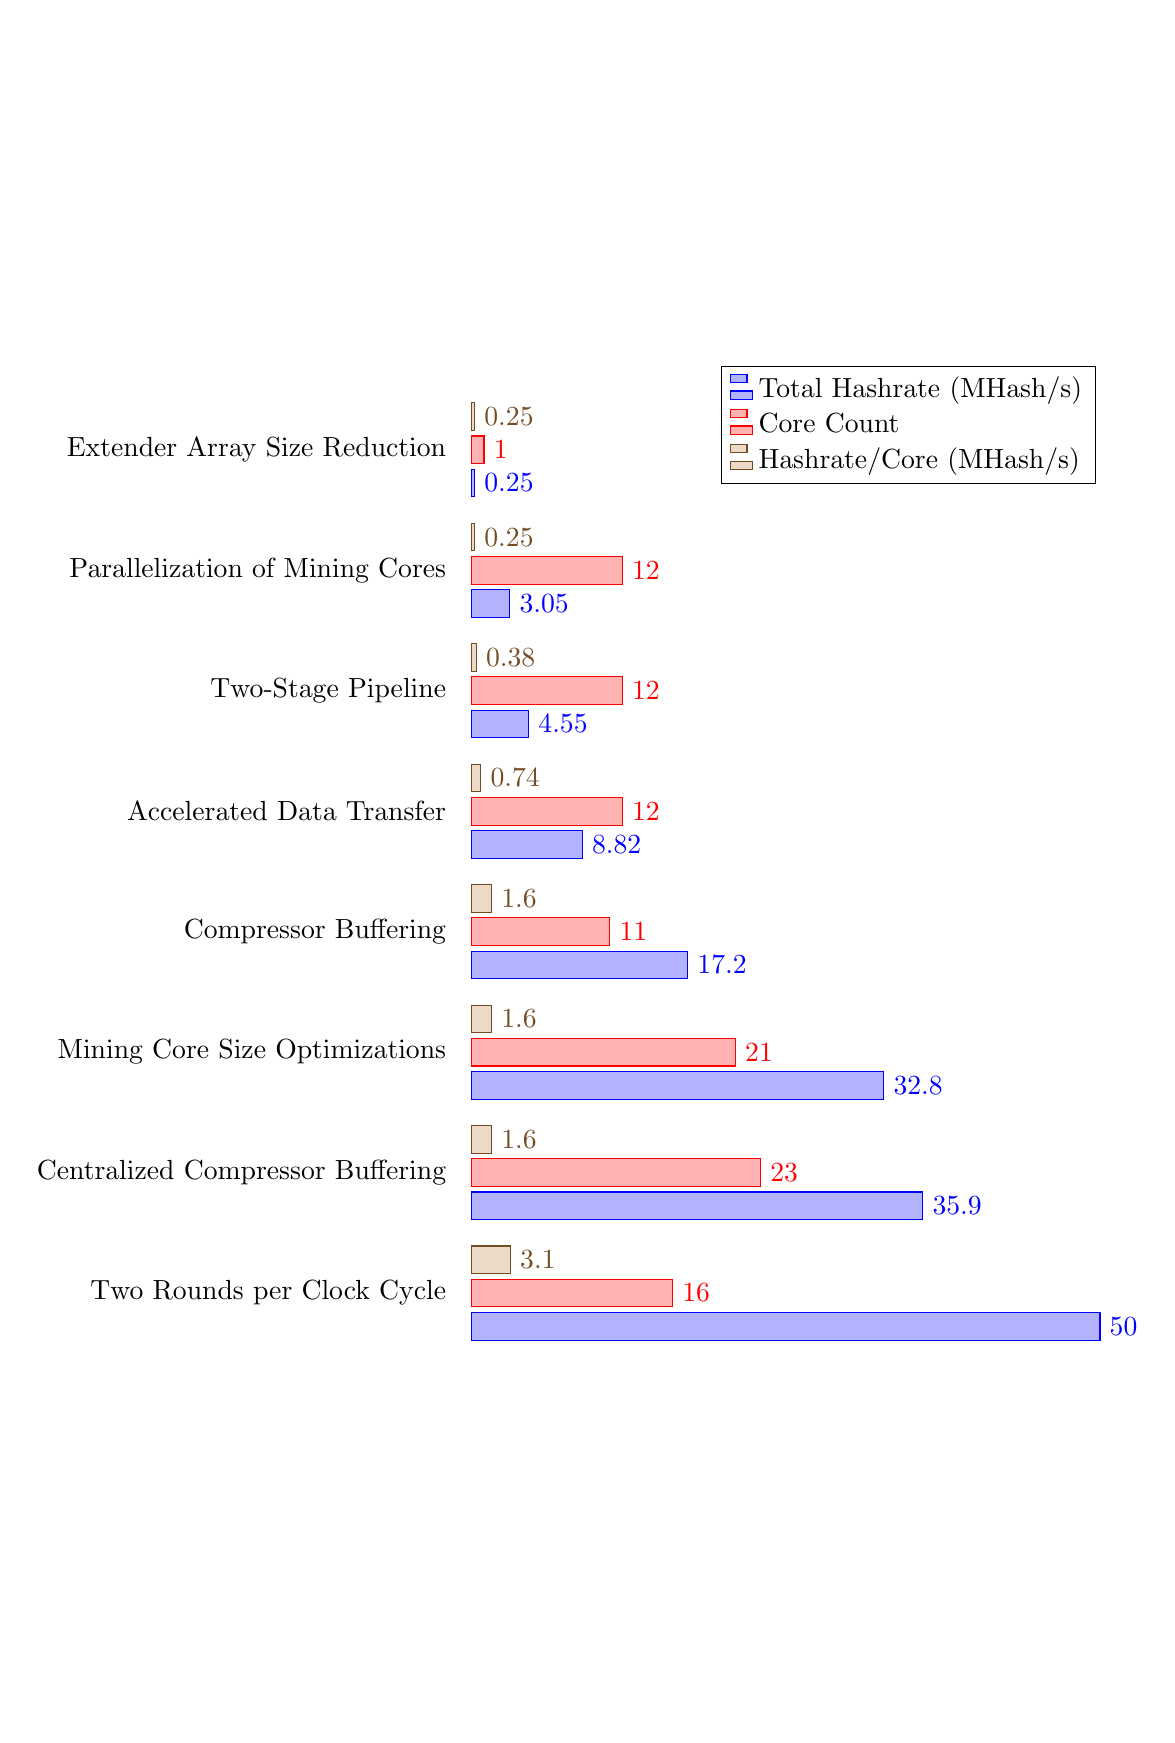
\begin{tikzpicture}
  \begin{axis}[
    xbar,
    y axis line style = { opacity = 0 },
    legend style={at={(0.4,0.8)},anchor=north west,nodes=right},
    axis x line       = none,
    tickwidth         = 0pt,
    enlarge y limits  = 0.5,
    enlarge x limits  = 0.03,
    ytick             = data,
    height            = 23cm,
    width             = 10cm,
    symbolic y coords = {Two Rounds per Clock Cycle, Centralized Compressor Buffering, Mining Core Size Optimizations, Compressor Buffering, Accelerated Data Transfer, Two-Stage Pipeline, Parallelization of Mining Cores, Extender Array Size Reduction},
    nodes near coords,
  ]
  \addplot coordinates { (0.25,Extender Array Size Reduction)(3.05,Parallelization of Mining Cores)(4.55,Two-Stage Pipeline)(8.82,Accelerated Data Transfer)(17.2,Compressor Buffering)(32.8,Mining Core Size Optimizations)(35.9,Centralized Compressor Buffering)(50.0,Two Rounds per Clock Cycle)};
  \addplot coordinates { (1,Extender Array Size Reduction)(12,Parallelization of Mining Cores)(12,Two-Stage Pipeline)(12,Accelerated Data Transfer)(11,Compressor Buffering)(21,Mining Core Size Optimizations)(23,Centralized Compressor Buffering)(16,Two Rounds per Clock Cycle)};
  \addplot coordinates { (0.25,Extender Array Size Reduction)(0.25,Parallelization of Mining Cores)(0.38,Two-Stage Pipeline)(0.74,Accelerated Data Transfer)(1.6,Compressor Buffering)(1.6,Mining Core Size Optimizations)(1.6,Centralized Compressor Buffering)(3.1,Two Rounds per Clock Cycle)};
  \legend{Total Hashrate (MHash/s), Core Count, Hashrate/Core (MHash/s)}
  \end{axis}
\end{tikzpicture}
\vspace*{-50mm}
\caption{Comparison of optimizations\label{Fig:optimizations}}
\end{figure}

%- https://gitlab.lrz.de/lrr-tum/students/eragp-blockchain-2020/-/commit/2af022551d0ddb0791a9bc34f254cb323b00f9ba/pipelines

\subsection{Comparison With Other Implementations}

%- Vergleich mit aktuellen Lösungen auf dem Markt hinsichtlich Performanz und auch Effizienz.
%- Vergleich aus bezüglich Wirtschaftlichkeit

In order to assess the significance of our implementation, it is crucial to compare its performance to other hardware. For this purpose we used a list provided by the bitcoin wiki\cite{bitcoinNonSpecializedHardware} \cite{bitcoinHardware}. As one can see from figure \ref{perf:hashrate} below, this paper shows, our implementation is capable to compete with CPUs and potentially GPUs with a larger FPGA board to host it. 
\begin{figure}
\centering

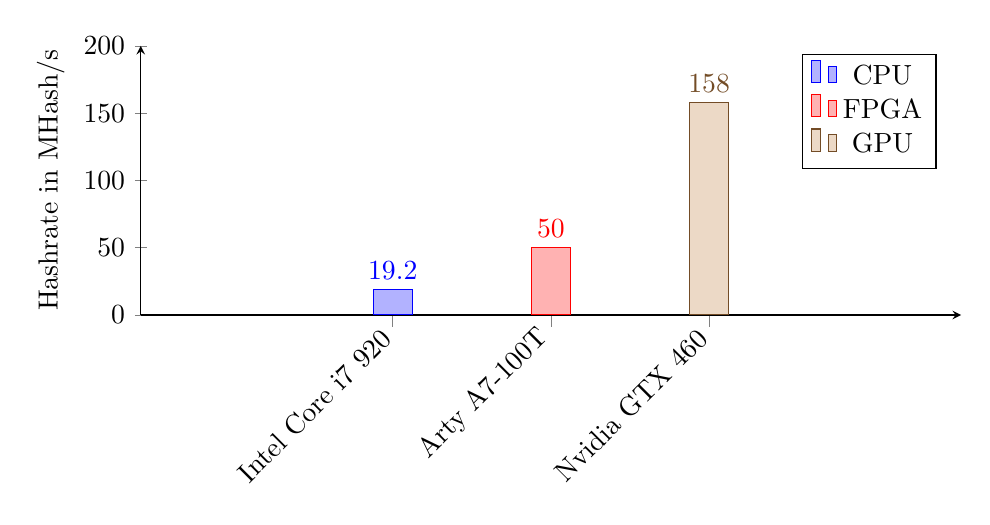
\begin{tikzpicture}
\pgfplotsset{width=10 cm}
\begin{axis} [
        symbolic x coords={Intel Core i7 920, Arty A7-100T, Nvidia GTX 460},
        xtick={Intel Core i7 920, Arty A7-100T, Nvidia GTX 460},
x tick label style={rotate=45, anchor=east, align=center},
axis lines=left,
ylabel={Hashrate in MHash/s},
legend style={at={(0.5,-0.10)},
    anchor=north,legend columns=1},
    ybar=0pt ,
    ymin=0,
    ymax=200,
    samples=2,
    width=12cm,
    height=5cm,
    domain=1:2,
    bar width=0.5cm,                       
    ybar=-0.5cm,                           
    enlarge x limits={abs=3.2cm},
    nodes near coords,                      
    nodes near coords align={vertical},  
    legend pos=north east  
]
     \addplot coordinates {(Intel Core i7 920, 19.2)};
     \addplot coordinates {(Arty A7-100T, 50.0)};
     \addplot coordinates {(Nvidia GTX 460, 158)};
      \legend{CPU, FPGA, GPU}

\end{axis}
\end{tikzpicture}
\caption{Comparison of hashrate of different hardware\label{perf:hashrate}}
\end{figure}
Unfortunately, this hashrate is minimal compared to that of an ASIC\footnote{This also explains the difficulty in finding mining data related to hardware more recent than the one presented here - due to the huge discrepancy in mining power between ASICs and other hardware, very few people still mine using CPUs and GPUs.}, as shown in figure \ref{perf:hashrateWAsic}, shedding strong doubt on the potential of FPGA implementations being able to compete with ASICs regarding cryptocurrency mining. 
\begin{figure}
\centering

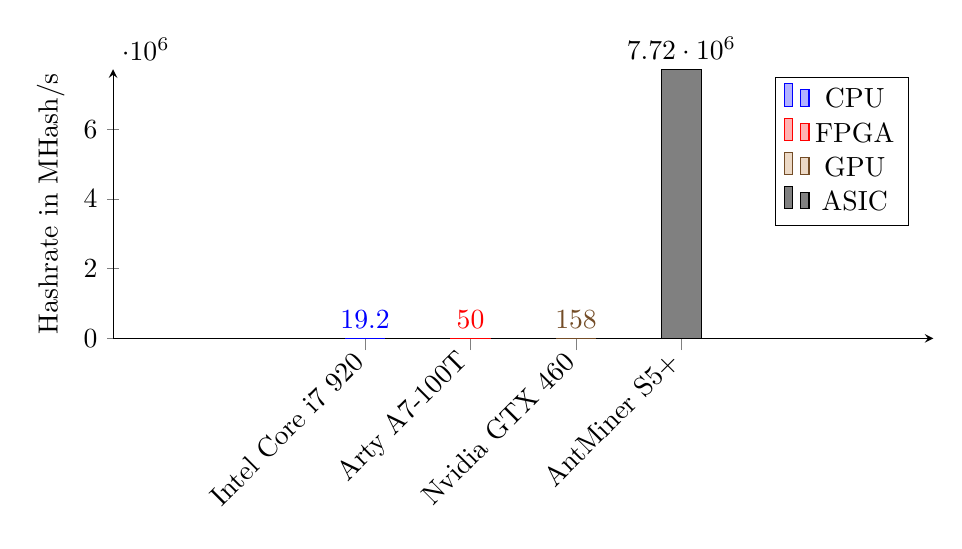
\begin{tikzpicture}
\pgfplotsset{width=10 cm}
\begin{axis} [
        symbolic x coords={Intel Core i7 920, Arty A7-100T, Nvidia GTX 460, AntMiner S5+},
        xtick={Intel Core i7 920, Arty A7-100T, Nvidia GTX 460,  AntMiner S5+},
x tick label style={rotate=45, anchor=east, align=center},
axis lines=left,
ylabel={Hashrate in MHash/s},
legend style={at={(0.5,-0.10)},
    anchor=north,legend columns=1},
    ybar=0pt ,
    ymin=0,
    ymax=7722000,
    samples=2,
    width=12cm,
    height=5cm,
    domain=1:2,
    bar width=0.5cm,                       
    ybar=-0.5cm,                           
    enlarge x limits={abs=3.2cm},
    nodes near coords,                      
    nodes near coords align={vertical},  
    legend pos=north east  
]
     \addplot coordinates {(Intel Core i7 920, 19.2)};
     \addplot coordinates {(Arty A7-100T, 50.0)};
     \addplot coordinates {(Nvidia GTX 460, 158)};
     \addplot coordinates {(AntMiner S5+, 7722000)};
     \legend{CPU, FPGA, GPU, ASIC}

\end{axis}
\end{tikzpicture}
\caption{Comparison of hashrate of different hardware including ASIC\label{perf:hashrateWAsic}}
\end{figure}


Another aspect to account for in Bitcoin mining is the power consumption of the specified hardware in relation to the hashrate generated. Upon first inspection in figure \ref{perf:efficiency}, our implementation shines, with nearly 30 times the efficiency of a GPU. 
\begin{figure}
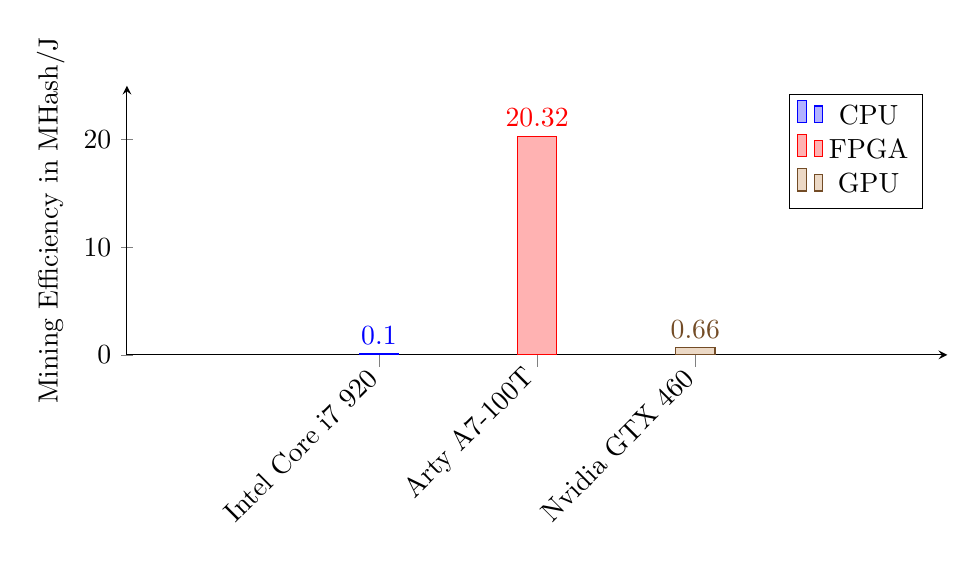
\begin{tikzpicture}
\pgfplotsset{width=10 cm}
\begin{axis} [
        symbolic x coords={Intel Core i7 920, Arty A7-100T, Nvidia GTX 460},
        xtick={Intel Core i7 920, Arty A7-100T, Nvidia GTX 460},
x tick label style={rotate=45, anchor=east, align=center},
axis lines=left,
ylabel={Mining Efficiency in MHash/J},
legend style={at={(0.5,-0.10)},
    anchor=north,legend columns=1},
    ybar=0pt ,
    ymin=0,
    ymax=25,
    samples=2,
    width=12cm,
    height=5cm,
    domain=1:2,
    bar width=0.5cm,                       
    ybar=-0.5cm,                           
    enlarge x limits={abs=3.2cm},
    nodes near coords,                      
    nodes near coords align={vertical},  
    legend pos=north east  
]
     \addplot coordinates {(Intel Core i7 920, 0.1)};
     \addplot coordinates {(Arty A7-100T, 20.32)};
     \addplot coordinates {(Nvidia GTX 460, 0.658)};
     \legend{CPU, FPGA, GPU}

\end{axis}
\end{tikzpicture}
\caption{Comparison of mining efficiency of different hardware\label{perf:efficiency}}
\end{figure}
Once again, however, the here described implementation cannot compete with the efficiency of an ASIC as depicted by figure ~\ref{perf:efficiencyWASIC}.


\begin{figure}
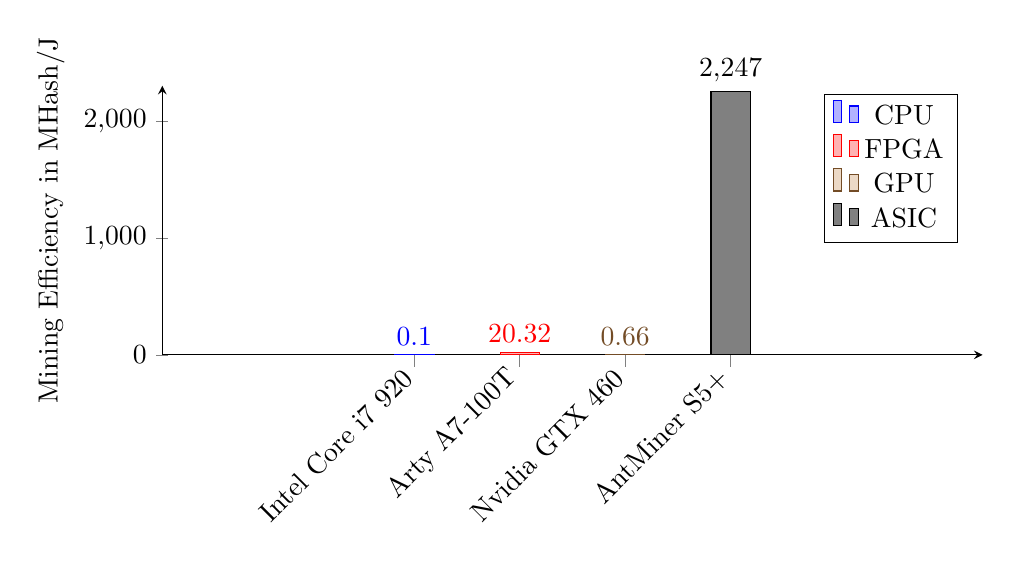
\begin{tikzpicture}
\pgfplotsset{width=10 cm}
\begin{axis} [
        symbolic x coords={Intel Core i7 920, Arty A7-100T, Nvidia GTX 460, AntMiner S5+},
        xtick={Intel Core i7 920, Arty A7-100T, Nvidia GTX 460,  AntMiner S5+},
x tick label style={rotate=45, anchor=east, align=center},
axis lines=left,
ylabel={Mining Efficiency in MHash/J},
legend style={at={(0.5,-0.10)},
    anchor=north,legend columns=1},
    ybar=0pt ,
    ymin=0,
    ymax=2300,
    samples=2,
    width=12cm,
    height=5cm,
    domain=1:2,
    bar width=0.5cm,                       
    ybar=-0.5cm,                           
    enlarge x limits={abs=3.2cm},
    nodes near coords,                      
    nodes near coords align={vertical},  
    legend pos=north east  
]
     \addplot coordinates {(Intel Core i7 920, 0.1)};
     \addplot coordinates {(Arty A7-100T, 20.32)};
     \addplot coordinates {(Nvidia GTX 460, 0.658)};
     \addplot coordinates {(AntMiner S5+, 2247)};
     \legend{CPU, FPGA, GPU, ASIC}

\end{axis}
\end{tikzpicture}
\caption{Comparison of mining efficiency of different hardware including ASIC\label{perf:efficiencyWASIC}}
\end{figure}

Additionally, it must be noted that the here-described implementation consumes 2.46 Watt regardless of whether it is computing useful hashes or calculating needless values while waiting for a new header. The power consumption was obtained from the static report generated by Vivado. The fact that the FPGA board might calculate needless hashes is acceptable in our use case, as the Bitcoin network has an uptime of $99.985\%$ and was last down in 2013. Therefore, we can rationally assume that a header will always be available to mine for the FPGA, making the time in which it is not calculating minimal. 

Now that we have estimated this implementation's electric efficiency, a final calculation that is of interest is the resulting economic efficiency. Therefore, we need the Bitcoin mining difficulty, which gives an indication of the difficulty to find a hash digest for the current target\footnote{More information on the Bitcoin mining difficulty can be found at \cite{bitcoinWikiDifficulty}}. The average time needed to find a block with a given hash rate H and mining difficulty D is $\frac{D \cdot 2^{32}}{H}$. At the time of this writing, the Bitcoin mining difficulty is $20.6 \cdot {10^{12}}$. Using this and our hash rate of $50.0$ MHash/s, we can simply estimate the time needed to find one valid block hash \cite{bitcoinWikiDifficulty}:

$t = \frac{20.6 \cdot {10^{12}} \cdot {2^{32}}} {5.00 \cdot {10^{7}}}$ seconds/block $\approx 1.77 \cdot {10^{15}}$ seconds/block $\approx 5.61 \cdot {10^{7}}$ years/block

At the time of this writing, the Bitcoin network rewards the miner with $6.25$ Bitcoin for mining a block. This means this implementation mines at a rate of $\frac{5.61 \cdot {10^{7}}}{6.25}$ years/bitcoin $\approx 8.98 \cdot {10^{6}}$ years/bitcoin $= 0.0898$ years/satoshi\footnote{Satoshi is the smallest piece to which a bitcoin can be broken down, with one bitcoin being equal to 100 million satoshi.}. Alternatively written, one can expect to make approximately $11.13$ satoshi/year. At the current Bitcoin price of $36.300$ USD, this is equal to approximately $0.004$ USD/year. However, these numbers do not account for the cost of electricity. Factoring this in, our implementation burns through $365.25 \cdot 24 \cdot 2.46 $ kWh/year $\approx 21.55$ kWh/year (with the power consumption of this implementation being $2.46 W$) if running full-time. The profitability of this implementation in dependence of the electricity price is visualized in graph \ref{perf:profitability}. Thus, the electricity price at which we break even is $1.86 \cdot {10^{-4}}$ USD/kWh.

\begin{figure}
\centering

\begin{tikzpicture}
\begin{axis}[xlabel=Price per kWh in USD,ylabel=Profit in USD,
xmin=0, xmax=0.0005,ymin=-0.005,ymax=0.005, axis lines=center]

\addplot[domain= 0:0.01, color=blue,]{0.004-21.55*x};

\end{axis}
\end{tikzpicture}
\caption{Profitabiliy depending on the price of electricity\label{perf:profitability}}
\end{figure}
